\subsection{Gate-based Quantum Computing}

In the gate-based model of quantum computers, gates represent the manipulation of qubits.
The qubits and quantum gates form a quantum circuit.

Single qubit gates manipulate only one qubit at a time.
Double qubit gates manipulate two qubits and can entangle two qubits.
The formula (\ref{formula:gate.x}) shows an example of a single qubit gate.
It swaps the amplitudes of the two basis states $\ket{0}$ and $\ket{1}$.
The formula (\ref{formula:gate.cnot}) shows an example of a double qubit gate.
It applies the $X$-gate to the second qubit if the first qubit is in the base state $\ket{1}$.
This entangles both qubits with each other.
\begin{subequations}
\begin{align}
  \label{formula:gate.x}
  X & = \ket{0} \bra{1} + \ket{1} \bra{0}
  & = \begin{pmatrix}
    0 & 1 \\ 1 & 0
  \end{pmatrix}
  \\
  \label{formula:gate.hadamard}
  H & = \frac{1}{\sqrt{2}} \left(
    \left( \ket{0} + \ket{1} \right) \bra{0}
    + \left( \ket{0} - \ket{1} \right) \bra{0}
  \right)
  & = \frac{1}{\sqrt{2}} \begin{pmatrix}
    1 & 1 \\ 1 & -1
  \end{pmatrix}
  \\
  \label{formula:gate.cnot}
  CNOT & = \ket{00} \bra{00} + \ket{01} \bra{01} + \ket{10} \bra{11} + \ket{11} \bra{10}
  & = \begin{pmatrix}
    1 & 0 & 0 & 0 \\
    0 & 1 & 0 & 0 \\
    0 & 0 & 0 & 1 \\
    0 & 0 & 1 & 0
  \end{pmatrix}
\end{align}
\end{subequations}

A quantum circuit consists of one or more quantum gates that are operating on one or more qubits.
The quantum circuit \ref{figure:gate.deutsch.circuit} depicts the Deutsch algorithm for the function $f: x \mapsto x$.
The dot with the line to the circled plus stands for the $CNOT$ gate, and the $H$ gates stand for Hadamard gates.
A Hadamard gate puts qubits that are in a basis state into a superposition where both outcomes of the measurement are equally likely.
It is described by the formula (\ref{formula:gate.hadamard}).
The last gate stands for a measurement.
In this case only the first qubit gets measured.
\cite{Deutsch1985}
\begin{figure}[!h]
  \centering
  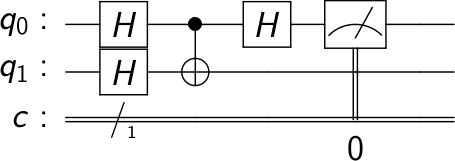
\includegraphics[width=0.5 \textwidth]{02_Background/deutsch_algorithm_circuit.png}
  \caption{Deutsch Algorithm for $f: x \mapsto x$}
  \label{figure:gate.deutsch.circuit}
\end{figure}

A quantum computer that implements this model of computing would be more powerful than any Turing machine.
It can simulate any finite physical system in polynomial time complexity, including systems with quantum effects.
The complexity class is called Bounded-error Quantum Polynomial-time (BQP).
There exists no algorithm for Turing machines to accomplish this.
%\cite{Shor1998}
